\documentclass[1p]{elsarticle_modified}
%\bibliographystyle{elsarticle-num}

%\usepackage[colorlinks]{hyperref}
%\usepackage{abbrmath_seonhwa} %\Abb, \Ascr, \Acal ,\Abf, \Afrak
\usepackage{amsfonts}
\usepackage{amssymb}
\usepackage{amsmath}
\usepackage{amsthm}
\usepackage{scalefnt}
\usepackage{amsbsy}
\usepackage{kotex}
\usepackage{caption}
\usepackage{subfig}
\usepackage{color}
\usepackage{graphicx}
\usepackage{xcolor} %% white, black, red, green, blue, cyan, magenta, yellow
\usepackage{float}
\usepackage{setspace}
\usepackage{hyperref}

\usepackage{tikz}
\usetikzlibrary{arrows}

\usepackage{multirow}
\usepackage{array} % fixed length table
\usepackage{hhline}

%%%%%%%%%%%%%%%%%%%%%
\makeatletter
\renewcommand*\env@matrix[1][\arraystretch]{%
	\edef\arraystretch{#1}%
	\hskip -\arraycolsep
	\let\@ifnextchar\new@ifnextchar
	\array{*\c@MaxMatrixCols c}}
\makeatother %https://tex.stackexchange.com/questions/14071/how-can-i-increase-the-line-spacing-in-a-matrix
%%%%%%%%%%%%%%%

\usepackage[normalem]{ulem}

\newcommand{\msout}[1]{\ifmmode\text{\sout{\ensuremath{#1}}}\else\sout{#1}\fi}
%SOURCE: \msout is \stkout macro in https://tex.stackexchange.com/questions/20609/strikeout-in-math-mode

\newcommand{\cancel}[1]{
	\ifmmode
	{\color{red}\msout{#1}}
	\else
	{\color{red}\sout{#1}}
	\fi
}

\newcommand{\add}[1]{
	{\color{blue}\uwave{#1}}
}

\newcommand{\replace}[2]{
	\ifmmode
	{\color{red}\msout{#1}}{\color{blue}\uwave{#2}}
	\else
	{\color{red}\sout{#1}}{\color{blue}\uwave{#2}}
	\fi
}

\newcommand{\Sol}{\mathcal{S}} %segment
\newcommand{\D}{D} %diagram
\newcommand{\A}{\mathcal{A}} %arc


%%%%%%%%%%%%%%%%%%%%%%%%%%%%%5 test

\def\sl{\operatorname{\textup{SL}}(2,\Cbb)}
\def\psl{\operatorname{\textup{PSL}}(2,\Cbb)}
\def\quan{\mkern 1mu \triangleright \mkern 1mu}

\theoremstyle{definition}
\newtheorem{thm}{Theorem}[section]
\newtheorem{prop}[thm]{Proposition}
\newtheorem{lem}[thm]{Lemma}
\newtheorem{ques}[thm]{Question}
\newtheorem{cor}[thm]{Corollary}
\newtheorem{defn}[thm]{Definition}
\newtheorem{exam}[thm]{Example}
\newtheorem{rmk}[thm]{Remark}
\newtheorem{alg}[thm]{Algorithm}

\newcommand{\I}{\sqrt{-1}}
\begin{document}

%\begin{frontmatter}
%
%\title{Boundary parabolic representations of knots up to 8 crossings}
%
%%% Group authors per affiliation:
%\author{Yunhi Cho} 
%\address{Department of Mathematics, University of Seoul, Seoul, Korea}
%\ead{yhcho@uos.ac.kr}
%
%
%\author{Seonhwa Kim} %\fnref{s_kim}}
%\address{Center for Geometry and Physics, Institute for Basic Science, Pohang, 37673, Korea}
%\ead{ryeona17@ibs.re.kr}
%
%\author{Hyuk Kim}
%\address{Department of Mathematical Sciences, Seoul National University, Seoul 08826, Korea}
%\ead{hyukkim@snu.ac.kr}
%
%\author{Seokbeom Yoon}
%\address{Department of Mathematical Sciences, Seoul National University, Seoul, 08826,  Korea}
%\ead{sbyoon15@snu.ac.kr}
%
%\begin{abstract}
%We find all boundary parabolic representation of knots up to 8 crossings.
%
%\end{abstract}
%\begin{keyword}
%    \MSC[2010] 57M25 
%\end{keyword}
%
%\end{frontmatter}

%\linenumbers
%\tableofcontents
%
\newcommand\colored[1]{\textcolor{white}{\rule[-0.35ex]{0.8em}{1.4ex}}\kern-0.8em\color{red} #1}%
%\newcommand\colored[1]{\textcolor{white}{ #1}\kern-2.17ex	\textcolor{white}{ #1}\kern-1.81ex	\textcolor{white}{ #1}\kern-2.15ex\color{red}#1	}

{\Large $\underline{12a_{0070}~(K12a_{0070})}$}

\setlength{\tabcolsep}{10pt}
\renewcommand{\arraystretch}{1.6}
\vspace{1cm}\begin{tabular}{m{100pt}>{\centering\arraybackslash}m{274pt}}
\multirow{5}{120pt}{
	\centering
	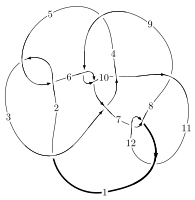
\includegraphics[width=112pt]{../../../GIT/diagram.site/Diagrams/png/871_12a_0070.png}\\
\ \ \ A knot diagram\footnotemark}&
\allowdisplaybreaks
\textbf{Linearized knot diagam} \\
\cline{2-2}
 &
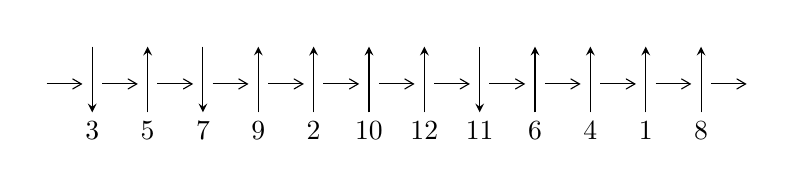
\begin{tikzpicture}[x=20pt, y=17pt]
	% nodes
	\node (C0) at (0, 0) {};
	\node (C1) at (1, 0) {};
	\node (C1U) at (1, +1) {};
	\node (C1D) at (1, -1) {3};

	\node (C2) at (2, 0) {};
	\node (C2U) at (2, +1) {};
	\node (C2D) at (2, -1) {5};

	\node (C3) at (3, 0) {};
	\node (C3U) at (3, +1) {};
	\node (C3D) at (3, -1) {7};

	\node (C4) at (4, 0) {};
	\node (C4U) at (4, +1) {};
	\node (C4D) at (4, -1) {9};

	\node (C5) at (5, 0) {};
	\node (C5U) at (5, +1) {};
	\node (C5D) at (5, -1) {2};

	\node (C6) at (6, 0) {};
	\node (C6U) at (6, +1) {};
	\node (C6D) at (6, -1) {10};

	\node (C7) at (7, 0) {};
	\node (C7U) at (7, +1) {};
	\node (C7D) at (7, -1) {12};

	\node (C8) at (8, 0) {};
	\node (C8U) at (8, +1) {};
	\node (C8D) at (8, -1) {11};

	\node (C9) at (9, 0) {};
	\node (C9U) at (9, +1) {};
	\node (C9D) at (9, -1) {6};

	\node (C10) at (10, 0) {};
	\node (C10U) at (10, +1) {};
	\node (C10D) at (10, -1) {4};

	\node (C11) at (11, 0) {};
	\node (C11U) at (11, +1) {};
	\node (C11D) at (11, -1) {1};

	\node (C12) at (12, 0) {};
	\node (C12U) at (12, +1) {};
	\node (C12D) at (12, -1) {8};
	\node (C13) at (13, 0) {};

	% arrows
	\draw[->,>={angle 60}]
	(C0) edge (C1) (C1) edge (C2) (C2) edge (C3) (C3) edge (C4) (C4) edge (C5) (C5) edge (C6) (C6) edge (C7) (C7) edge (C8) (C8) edge (C9) (C9) edge (C10) (C10) edge (C11) (C11) edge (C12) (C12) edge (C13) ;	\draw[->,>=stealth]
	(C1U) edge (C1D) (C2D) edge (C2U) (C3U) edge (C3D) (C4D) edge (C4U) (C5D) edge (C5U) (C6D) edge (C6U) (C7D) edge (C7U) (C8U) edge (C8D) (C9D) edge (C9U) (C10D) edge (C10U) (C11D) edge (C11U) (C12D) edge (C12U) ;
	\end{tikzpicture} \\
\hhline{~~} \\& 
\textbf{Solving Sequence} \\ \cline{2-2} 
 &
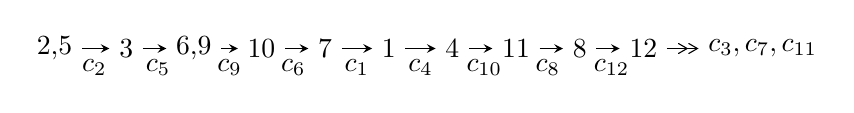
\begin{tikzpicture}[x=23pt, y=7pt]
	% node
	\node (A0) at (-1/8, 0) {2,5};
	\node (A1) at (1, 0) {3};
	\node (A2) at (33/16, 0) {6,9};
	\node (A3) at (25/8, 0) {10};
	\node (A4) at (33/8, 0) {7};
	\node (A5) at (41/8, 0) {1};
	\node (A6) at (49/8, 0) {4};
	\node (A7) at (57/8, 0) {11};
	\node (A8) at (65/8, 0) {8};
	\node (A9) at (73/8, 0) {12};
	\node (C1) at (1/2, -1) {$c_{2}$};
	\node (C2) at (3/2, -1) {$c_{5}$};
	\node (C3) at (21/8, -1) {$c_{9}$};
	\node (C4) at (29/8, -1) {$c_{6}$};
	\node (C5) at (37/8, -1) {$c_{1}$};
	\node (C6) at (45/8, -1) {$c_{4}$};
	\node (C7) at (53/8, -1) {$c_{10}$};
	\node (C8) at (61/8, -1) {$c_{8}$};
	\node (C9) at (69/8, -1) {$c_{12}$};
	\node (A10) at (11, 0) {$c_{3},c_{7},c_{11}$};

	% edge
	\draw[->,>=stealth]	
	(A0) edge (A1) (A1) edge (A2) (A2) edge (A3) (A3) edge (A4) (A4) edge (A5) (A5) edge (A6) (A6) edge (A7) (A7) edge (A8) (A8) edge (A9) ;
	\draw[->>,>={angle 60}]	
	(A9) edge (A10);
\end{tikzpicture} \\ 

\end{tabular} \\

\footnotetext{
The image of knot diagram is generated by the software ``\textbf{Draw programme}" developed by Andrew Bartholomew(\url{http://www.layer8.co.uk/maths/draw/index.htm\#Running-draw}), where we modified some parts for our purpose(\url{https://github.com/CATsTAILs/LinksPainter}).
}\phantom \\ \newline 
\centering \textbf{Ideals for irreducible components\footnotemark of $X_{\text{par}}$} 
 
\begin{align*}
I^u_{1}&=\langle 
-4.73994\times10^{281} u^{121}+1.62267\times10^{282} u^{120}+\cdots+4.12994\times10^{281} b+5.77778\times10^{282},\\
\phantom{I^u_{1}}&\phantom{= \langle  }-2.42748\times10^{282} u^{121}+8.21343\times10^{282} u^{120}+\cdots+2.06497\times10^{282} a+9.97461\times10^{282},\\
\phantom{I^u_{1}}&\phantom{= \langle  }u^{122}-4 u^{121}+\cdots+199 u+25\rangle \\
I^u_{2}&=\langle 
-10 a^2+13 a u+5 b-5 a+u+1,\;5 a^3-4 a^2 u- a u- a-1,\;u^2+u+1\rangle \\
\\
\end{align*}
\raggedright * 2 irreducible components of $\dim_{\mathbb{C}}=0$, with total 128 representations.\\
\footnotetext{All coefficients of polynomials are rational numbers. But the coefficients are sometimes approximated in decimal forms when there is not enough margin.}
\newpage
\renewcommand{\arraystretch}{1}
\centering \section*{I. $I^u_{1}= \langle -4.74\times10^{281} u^{121}+1.62\times10^{282} u^{120}+\cdots+4.13\times10^{281} b+5.78\times10^{282},\;-2.43\times10^{282} u^{121}+8.21\times10^{282} u^{120}+\cdots+2.06\times10^{282} a+9.97\times10^{282},\;u^{122}-4 u^{121}+\cdots+199 u+25 \rangle$}
\flushleft \textbf{(i) Arc colorings}\\
\begin{tabular}{m{7pt} m{180pt} m{7pt} m{180pt} }
\flushright $a_{2}=$&$\begin{pmatrix}1\\0\end{pmatrix}$ \\
\flushright $a_{5}=$&$\begin{pmatrix}0\\u\end{pmatrix}$ \\
\flushright $a_{3}=$&$\begin{pmatrix}1\\- u^2\end{pmatrix}$ \\
\flushright $a_{6}=$&$\begin{pmatrix}u\\u\end{pmatrix}$ \\
\flushright $a_{9}=$&$\begin{pmatrix}1.17555 u^{121}-3.97750 u^{120}+\cdots-47.5754 u-4.83038\\1.14770 u^{121}-3.92903 u^{120}+\cdots-111.438 u-13.9900\end{pmatrix}$ \\
\flushright $a_{10}=$&$\begin{pmatrix}0.869037 u^{121}-3.13754 u^{120}+\cdots-34.3561 u-3.25714\\0.841186 u^{121}-3.08907 u^{120}+\cdots-98.2189 u-12.4167\end{pmatrix}$ \\
\flushright $a_{7}=$&$\begin{pmatrix}1.25220 u^{121}-4.99677 u^{120}+\cdots-279.917 u-36.4053\\1.16763 u^{121}-2.48554 u^{120}+\cdots+149.063 u+13.0091\end{pmatrix}$ \\
\flushright $a_{1}=$&$\begin{pmatrix}u^2+1\\- u^4\end{pmatrix}$ \\
\flushright $a_{4}=$&$\begin{pmatrix}0.134051 u^{121}+0.485797 u^{120}+\cdots+72.7723 u+10.5439\\-1.71953 u^{121}+6.19096 u^{120}+\cdots+223.156 u+28.4621\end{pmatrix}$ \\
\flushright $a_{11}=$&$\begin{pmatrix}-0.0930748 u^{121}+0.186740 u^{120}+\cdots-25.6459 u-1.79576\\0.0179185 u^{121}-0.626037 u^{120}+\cdots-119.121 u-13.9132\end{pmatrix}$ \\
\flushright $a_{8}=$&$\begin{pmatrix}-0.823254 u^{121}+3.23286 u^{120}+\cdots+200.194 u+26.4359\\-0.969644 u^{121}+2.62640 u^{120}+\cdots-8.27264 u+1.68771\end{pmatrix}$ \\
\flushright $a_{12}=$&$\begin{pmatrix}-0.622433 u^{121}+2.11008 u^{120}+\cdots+58.1543 u+8.71432\\-0.615775 u^{121}+1.57164 u^{120}+\cdots-49.5573 u-4.66944\end{pmatrix}$\\&\end{tabular}
\flushleft \textbf{(ii) Obstruction class $= -1$}\\~\\
\flushleft \textbf{(iii) Cusp Shapes $= -0.314772 u^{121}+1.38514 u^{120}+\cdots+51.9020 u+17.1153$}\\~\\
\newpage\renewcommand{\arraystretch}{1}
\flushleft \textbf{(iv) u-Polynomials at the component}\newline \\
\begin{tabular}{m{50pt}|m{274pt}}
Crossings & \hspace{64pt}u-Polynomials at each crossing \\
\hline $$\begin{aligned}c_{1}\end{aligned}$$&$\begin{aligned}
&u^{122}+44 u^{121}+\cdots-11251 u+625
\end{aligned}$\\
\hline $$\begin{aligned}c_{2},c_{5}\end{aligned}$$&$\begin{aligned}
&u^{122}+4 u^{121}+\cdots-199 u+25
\end{aligned}$\\
\hline $$\begin{aligned}c_{3}\end{aligned}$$&$\begin{aligned}
&25(25 u^{122}-110 u^{121}+\cdots-2.01822\times10^{8} u+2.90241\times10^{7})
\end{aligned}$\\
\hline $$\begin{aligned}c_{4}\end{aligned}$$&$\begin{aligned}
&25(25 u^{122}+285 u^{121}+\cdots+1.39320\times10^{8} u-4.70438\times10^{8})
\end{aligned}$\\
\hline $$\begin{aligned}c_{6},c_{9}\end{aligned}$$&$\begin{aligned}
&u^{122}-3 u^{121}+\cdots+6 u-1
\end{aligned}$\\
\hline $$\begin{aligned}c_{7},c_{12}\end{aligned}$$&$\begin{aligned}
&u^{122}-3 u^{121}+\cdots+2 u-1
\end{aligned}$\\
\hline $$\begin{aligned}c_{8}\end{aligned}$$&$\begin{aligned}
&u^{122}-9 u^{121}+\cdots+464382 u-40851
\end{aligned}$\\
\hline $$\begin{aligned}c_{10}\end{aligned}$$&$\begin{aligned}
&u^{122}-3 u^{121}+\cdots-64800 u+8000
\end{aligned}$\\
\hline $$\begin{aligned}c_{11}\end{aligned}$$&$\begin{aligned}
&u^{122}-61 u^{121}+\cdots-6 u+1
\end{aligned}$\\
\hline
\end{tabular}\\~\\
\newpage\renewcommand{\arraystretch}{1}
\flushleft \textbf{(v) Riley Polynomials at the component}\newline \\
\begin{tabular}{m{50pt}|m{274pt}}
Crossings & \hspace{64pt}Riley Polynomials at each crossing \\
\hline $$\begin{aligned}c_{1}\end{aligned}$$&$\begin{aligned}
&y^{122}+72 y^{121}+\cdots-671351251 y+390625
\end{aligned}$\\
\hline $$\begin{aligned}c_{2},c_{5}\end{aligned}$$&$\begin{aligned}
&y^{122}+44 y^{121}+\cdots-11251 y+625
\end{aligned}$\\
\hline $$\begin{aligned}c_{3}\end{aligned}$$&$\begin{aligned}
&625(625 y^{122}+33050 y^{121}+\cdots+9.83882\times10^{15} y+8.42397\times10^{14})
\end{aligned}$\\
\hline $$\begin{aligned}c_{4}\end{aligned}$$&$\begin{aligned}
&625(625 y^{122}-37825 y^{121}+\cdots-5.31980\times10^{18} y+2.21312\times10^{17})
\end{aligned}$\\
\hline $$\begin{aligned}c_{6},c_{9}\end{aligned}$$&$\begin{aligned}
&y^{122}-77 y^{121}+\cdots-6 y+1
\end{aligned}$\\
\hline $$\begin{aligned}c_{7},c_{12}\end{aligned}$$&$\begin{aligned}
&y^{122}-61 y^{121}+\cdots-6 y+1
\end{aligned}$\\
\hline $$\begin{aligned}c_{8}\end{aligned}$$&$\begin{aligned}
&y^{122}+55 y^{121}+\cdots-105170828166 y+1668804201
\end{aligned}$\\
\hline $$\begin{aligned}c_{10}\end{aligned}$$&$\begin{aligned}
&y^{122}-35 y^{121}+\cdots-1976960000 y+64000000
\end{aligned}$\\
\hline $$\begin{aligned}c_{11}\end{aligned}$$&$\begin{aligned}
&y^{122}+3 y^{121}+\cdots-26 y+1
\end{aligned}$\\
\hline
\end{tabular}\\~\\
\newpage\flushleft \textbf{(vi) Complex Volumes and Cusp Shapes}
$$\begin{array}{c|c|c}  
\text{Solutions to }I^u_{1}& \I (\text{vol} + \sqrt{-1}CS) & \text{Cusp shape}\\
 \hline 
\begin{aligned}
u &= \phantom{-}0.326285 + 0.942418 I \\
a &= \phantom{-}0.692847 + 0.187568 I \\
b &= \phantom{-}1.78757 + 0.05136 I\end{aligned}
 & -3.66042 + 5.13633 I & \phantom{-0.000000 } 0 \\ \hline\begin{aligned}
u &= \phantom{-}0.326285 - 0.942418 I \\
a &= \phantom{-}0.692847 - 0.187568 I \\
b &= \phantom{-}1.78757 - 0.05136 I\end{aligned}
 & -3.66042 - 5.13633 I & \phantom{-0.000000 } 0 \\ \hline\begin{aligned}
u &= -0.572010 + 0.816257 I \\
a &= \phantom{-}0.507803 - 0.572524 I \\
b &= \phantom{-}0.260550 - 0.686004 I\end{aligned}
 & \phantom{-}0.73647 - 2.28933 I & \phantom{-0.000000 } 0 \\ \hline\begin{aligned}
u &= -0.572010 - 0.816257 I \\
a &= \phantom{-}0.507803 + 0.572524 I \\
b &= \phantom{-}0.260550 + 0.686004 I\end{aligned}
 & \phantom{-}0.73647 + 2.28933 I & \phantom{-0.000000 } 0 \\ \hline\begin{aligned}
u &= \phantom{-}0.553016 + 0.850381 I \\
a &= -0.437624 + 0.409552 I \\
b &= -1.53016 - 0.57476 I\end{aligned}
 & -2.78287 - 0.75215 I & \phantom{-0.000000 } 0 \\ \hline\begin{aligned}
u &= \phantom{-}0.553016 - 0.850381 I \\
a &= -0.437624 - 0.409552 I \\
b &= -1.53016 + 0.57476 I\end{aligned}
 & -2.78287 + 0.75215 I & \phantom{-0.000000 } 0 \\ \hline\begin{aligned}
u &= \phantom{-}0.218439 + 0.992336 I \\
a &= -0.799538 - 0.333829 I \\
b &= -1.69967 - 0.12677 I\end{aligned}
 & -4.61287 + 0.09185 I & \phantom{-0.000000 } 0 \\ \hline\begin{aligned}
u &= \phantom{-}0.218439 - 0.992336 I \\
a &= -0.799538 + 0.333829 I \\
b &= -1.69967 + 0.12677 I\end{aligned}
 & -4.61287 - 0.09185 I & \phantom{-0.000000 } 0 \\ \hline\begin{aligned}
u &= \phantom{-}0.795450 + 0.578520 I \\
a &= \phantom{-}0.373619 - 1.026800 I \\
b &= \phantom{-}0.839001 - 0.103657 I\end{aligned}
 & \phantom{-}4.78667 - 7.85752 I & \phantom{-0.000000 } 0 \\ \hline\begin{aligned}
u &= \phantom{-}0.795450 - 0.578520 I \\
a &= \phantom{-}0.373619 + 1.026800 I \\
b &= \phantom{-}0.839001 + 0.103657 I\end{aligned}
 & \phantom{-}4.78667 + 7.85752 I & \phantom{-0.000000 } 0\\
 \hline 
 \end{array}$$\newpage$$\begin{array}{c|c|c}  
\text{Solutions to }I^u_{1}& \I (\text{vol} + \sqrt{-1}CS) & \text{Cusp shape}\\
 \hline 
\begin{aligned}
u &= -0.529652 + 0.820417 I \\
a &= -1.76543 + 3.76659 I \\
b &= -2.39046 + 2.84255 I\end{aligned}
 & \phantom{-}1.90583 - 1.93557 I & \phantom{-0.000000 } 0 \\ \hline\begin{aligned}
u &= -0.529652 - 0.820417 I \\
a &= -1.76543 - 3.76659 I \\
b &= -2.39046 - 2.84255 I\end{aligned}
 & \phantom{-}1.90583 + 1.93557 I & \phantom{-0.000000 } 0 \\ \hline\begin{aligned}
u &= \phantom{-}0.749029 + 0.701395 I \\
a &= \phantom{-}0.469358 - 0.870420 I \\
b &= \phantom{-}1.055920 + 0.011491 I\end{aligned}
 & \phantom{-}6.29582 + 1.05570 I & \phantom{-0.000000 } 0 \\ \hline\begin{aligned}
u &= \phantom{-}0.749029 - 0.701395 I \\
a &= \phantom{-}0.469358 + 0.870420 I \\
b &= \phantom{-}1.055920 - 0.011491 I\end{aligned}
 & \phantom{-}6.29582 - 1.05570 I & \phantom{-0.000000 } 0 \\ \hline\begin{aligned}
u &= -0.510762 + 0.914144 I \\
a &= -3.17676 - 1.26449 I \\
b &= -3.73598 - 2.07584 I\end{aligned}
 & \phantom{-}1.59606 - 2.27047 I & \phantom{-0.000000 } 0 \\ \hline\begin{aligned}
u &= -0.510762 - 0.914144 I \\
a &= -3.17676 + 1.26449 I \\
b &= -3.73598 + 2.07584 I\end{aligned}
 & \phantom{-}1.59606 + 2.27047 I & \phantom{-0.000000 } 0 \\ \hline\begin{aligned}
u &= \phantom{-}0.779251 + 0.539024 I \\
a &= \phantom{-}0.58932 - 1.31309 I \\
b &= -0.381525 - 0.131833 I\end{aligned}
 & \phantom{-}3.36722 - 6.19016 I & \phantom{-0.000000 } 0 \\ \hline\begin{aligned}
u &= \phantom{-}0.779251 - 0.539024 I \\
a &= \phantom{-}0.58932 + 1.31309 I \\
b &= -0.381525 + 0.131833 I\end{aligned}
 & \phantom{-}3.36722 + 6.19016 I & \phantom{-0.000000 } 0 \\ \hline\begin{aligned}
u &= \phantom{-}0.724387 + 0.597756 I \\
a &= -0.332312 + 0.938470 I \\
b &= -0.850470 - 0.028516 I\end{aligned}
 & \phantom{-}1.82069 - 2.81316 I & \phantom{-0.000000 } 0 \\ \hline\begin{aligned}
u &= \phantom{-}0.724387 - 0.597756 I \\
a &= -0.332312 - 0.938470 I \\
b &= -0.850470 + 0.028516 I\end{aligned}
 & \phantom{-}1.82069 + 2.81316 I & \phantom{-0.000000 } 0\\
 \hline 
 \end{array}$$\newpage$$\begin{array}{c|c|c}  
\text{Solutions to }I^u_{1}& \I (\text{vol} + \sqrt{-1}CS) & \text{Cusp shape}\\
 \hline 
\begin{aligned}
u &= -0.242829 + 1.033120 I \\
a &= \phantom{-}0.789327 + 0.692107 I \\
b &= \phantom{-}1.194330 + 0.413124 I\end{aligned}
 & \phantom{-}0.308045 + 0.406265 I & \phantom{-0.000000 } 0 \\ \hline\begin{aligned}
u &= -0.242829 - 1.033120 I \\
a &= \phantom{-}0.789327 - 0.692107 I \\
b &= \phantom{-}1.194330 - 0.413124 I\end{aligned}
 & \phantom{-}0.308045 - 0.406265 I & \phantom{-0.000000 } 0 \\ \hline\begin{aligned}
u &= \phantom{-}0.559214 + 0.903189 I \\
a &= \phantom{-}0.571243 - 0.340975 I \\
b &= \phantom{-}1.71545 + 0.36241 I\end{aligned}
 & -2.96199 + 5.17216 I & \phantom{-0.000000 } 0 \\ \hline\begin{aligned}
u &= \phantom{-}0.559214 - 0.903189 I \\
a &= \phantom{-}0.571243 + 0.340975 I \\
b &= \phantom{-}1.71545 - 0.36241 I\end{aligned}
 & -2.96199 - 5.17216 I & \phantom{-0.000000 } 0 \\ \hline\begin{aligned}
u &= \phantom{-}0.026443 + 1.069990 I \\
a &= -0.909170 - 0.542272 I \\
b &= -1.56204 - 0.29348 I\end{aligned}
 & -3.43542 - 1.88104 I & \phantom{-0.000000 } 0 \\ \hline\begin{aligned}
u &= \phantom{-}0.026443 - 1.069990 I \\
a &= -0.909170 + 0.542272 I \\
b &= -1.56204 + 0.29348 I\end{aligned}
 & -3.43542 + 1.88104 I & \phantom{-0.000000 } 0 \\ \hline\begin{aligned}
u &= \phantom{-}0.681014 + 0.619625 I \\
a &= -0.438429 + 1.272400 I \\
b &= \phantom{-}0.446348 - 0.085207 I\end{aligned}
 & \phantom{-}2.94385 - 1.10084 I & \phantom{-0.000000 } 0 \\ \hline\begin{aligned}
u &= \phantom{-}0.681014 - 0.619625 I \\
a &= -0.438429 - 1.272400 I \\
b &= \phantom{-}0.446348 + 0.085207 I\end{aligned}
 & \phantom{-}2.94385 + 1.10084 I & \phantom{-0.000000 } 0 \\ \hline\begin{aligned}
u &= \phantom{-}0.078954 + 1.079210 I \\
a &= -0.314714 - 0.213547 I \\
b &= -0.711670 - 1.188950 I\end{aligned}
 & -1.82843 - 0.11722 I & \phantom{-0.000000 } 0 \\ \hline\begin{aligned}
u &= \phantom{-}0.078954 - 1.079210 I \\
a &= -0.314714 + 0.213547 I \\
b &= -0.711670 + 1.188950 I\end{aligned}
 & -1.82843 + 0.11722 I & \phantom{-0.000000 } 0\\
 \hline 
 \end{array}$$\newpage$$\begin{array}{c|c|c}  
\text{Solutions to }I^u_{1}& \I (\text{vol} + \sqrt{-1}CS) & \text{Cusp shape}\\
 \hline 
\begin{aligned}
u &= \phantom{-}0.713590 + 0.819160 I \\
a &= -0.549865 + 0.433932 I \\
b &= -1.82136 + 0.96114 I\end{aligned}
 & \phantom{-}8.11043 - 1.78541 I & \phantom{-0.000000 } 0 \\ \hline\begin{aligned}
u &= \phantom{-}0.713590 - 0.819160 I \\
a &= -0.549865 - 0.433932 I \\
b &= -1.82136 - 0.96114 I\end{aligned}
 & \phantom{-}8.11043 + 1.78541 I & \phantom{-0.000000 } 0 \\ \hline\begin{aligned}
u &= \phantom{-}0.691033 + 0.838832 I \\
a &= -0.458451 + 0.897802 I \\
b &= \phantom{-}0.058154 - 0.460882 I\end{aligned}
 & \phantom{-}5.24954 + 1.80028 I & \phantom{-0.000000 } 0 \\ \hline\begin{aligned}
u &= \phantom{-}0.691033 - 0.838832 I \\
a &= -0.458451 - 0.897802 I \\
b &= \phantom{-}0.058154 + 0.460882 I\end{aligned}
 & \phantom{-}5.24954 - 1.80028 I & \phantom{-0.000000 } 0 \\ \hline\begin{aligned}
u &= -0.912021\phantom{ +0.000000I} \\
a &= -1.22780\phantom{ +0.000000I} \\
b &= \phantom{-}0.0961263\phantom{ +0.000000I}\end{aligned}
 & \phantom{-}5.29705\phantom{ +0.000000I} & \phantom{-0.000000 } 0 \\ \hline\begin{aligned}
u &= -0.425723 + 0.799219 I \\
a &= -1.38513 - 4.06579 I \\
b &= -0.84055 - 2.95736 I\end{aligned}
 & \phantom{-}3.93682 + 1.93972 I & \phantom{-0.000000 } 0 \\ \hline\begin{aligned}
u &= -0.425723 - 0.799219 I \\
a &= -1.38513 + 4.06579 I \\
b &= -0.84055 + 2.95736 I\end{aligned}
 & \phantom{-}3.93682 - 1.93972 I & \phantom{-0.000000 } 0 \\ \hline\begin{aligned}
u &= -0.433038 + 1.007040 I \\
a &= -0.496728 - 0.724378 I \\
b &= -0.773503 - 0.549607 I\end{aligned}
 & -0.87402 - 2.91759 I & \phantom{-0.000000 } 0 \\ \hline\begin{aligned}
u &= -0.433038 - 1.007040 I \\
a &= -0.496728 + 0.724378 I \\
b &= -0.773503 + 0.549607 I\end{aligned}
 & -0.87402 + 2.91759 I & \phantom{-0.000000 } 0 \\ \hline\begin{aligned}
u &= \phantom{-}0.689166 + 0.869505 I \\
a &= \phantom{-}0.662720 - 0.365295 I \\
b &= \phantom{-}1.90462 - 0.97010 I\end{aligned}
 & \phantom{-}5.15598 + 3.50593 I & \phantom{-0.000000 } 0\\
 \hline 
 \end{array}$$\newpage$$\begin{array}{c|c|c}  
\text{Solutions to }I^u_{1}& \I (\text{vol} + \sqrt{-1}CS) & \text{Cusp shape}\\
 \hline 
\begin{aligned}
u &= \phantom{-}0.689166 - 0.869505 I \\
a &= \phantom{-}0.662720 + 0.365295 I \\
b &= \phantom{-}1.90462 + 0.97010 I\end{aligned}
 & \phantom{-}5.15598 - 3.50593 I & \phantom{-0.000000 } 0 \\ \hline\begin{aligned}
u &= \phantom{-}0.957418 + 0.574316 I \\
a &= \phantom{-}0.71742 - 1.26333 I \\
b &= -0.137405 - 0.288808 I\end{aligned}
 & \phantom{-}6.71552 - 7.89088 I & \phantom{-0.000000 } 0 \\ \hline\begin{aligned}
u &= \phantom{-}0.957418 - 0.574316 I \\
a &= \phantom{-}0.71742 + 1.26333 I \\
b &= -0.137405 + 0.288808 I\end{aligned}
 & \phantom{-}6.71552 + 7.89088 I & \phantom{-0.000000 } 0 \\ \hline\begin{aligned}
u &= -0.501781 + 0.723894 I \\
a &= -2.66535 + 0.96560 I \\
b &= -2.19693 + 1.68940 I\end{aligned}
 & \phantom{-}4.16095 - 5.28585 I & \phantom{-0.000000 } 0 \\ \hline\begin{aligned}
u &= -0.501781 - 0.723894 I \\
a &= -2.66535 - 0.96560 I \\
b &= -2.19693 - 1.68940 I\end{aligned}
 & \phantom{-}4.16095 + 5.28585 I & \phantom{-0.000000 } 0 \\ \hline\begin{aligned}
u &= \phantom{-}0.777934 + 0.809289 I \\
a &= \phantom{-}0.577136 - 0.989100 I \\
b &= -0.008776 + 0.238221 I\end{aligned}
 & \phantom{-}10.29660 - 1.59255 I & \phantom{-0.000000 } 0 \\ \hline\begin{aligned}
u &= \phantom{-}0.777934 - 0.809289 I \\
a &= \phantom{-}0.577136 + 0.989100 I \\
b &= -0.008776 - 0.238221 I\end{aligned}
 & \phantom{-}10.29660 + 1.59255 I & \phantom{-0.000000 } 0 \\ \hline\begin{aligned}
u &= \phantom{-}0.699861 + 0.892444 I \\
a &= \phantom{-}0.514457 - 0.817381 I \\
b &= \phantom{-}0.086762 + 0.498270 I\end{aligned}
 & \phantom{-}7.88589 + 7.19296 I & \phantom{-0.000000 } 0 \\ \hline\begin{aligned}
u &= \phantom{-}0.699861 - 0.892444 I \\
a &= \phantom{-}0.514457 + 0.817381 I \\
b &= \phantom{-}0.086762 - 0.498270 I\end{aligned}
 & \phantom{-}7.88589 - 7.19296 I & \phantom{-0.000000 } 0 \\ \hline\begin{aligned}
u &= -0.020184 + 1.138770 I \\
a &= \phantom{-}0.965921 + 0.597820 I \\
b &= \phantom{-}1.55915 + 0.39430 I\end{aligned}
 & -1.16117 - 6.62977 I & \phantom{-0.000000 } 0\\
 \hline 
 \end{array}$$\newpage$$\begin{array}{c|c|c}  
\text{Solutions to }I^u_{1}& \I (\text{vol} + \sqrt{-1}CS) & \text{Cusp shape}\\
 \hline 
\begin{aligned}
u &= -0.020184 - 1.138770 I \\
a &= \phantom{-}0.965921 - 0.597820 I \\
b &= \phantom{-}1.55915 - 0.39430 I\end{aligned}
 & -1.16117 + 6.62977 I & \phantom{-0.000000 } 0 \\ \hline\begin{aligned}
u &= \phantom{-}0.953494 + 0.635428 I \\
a &= -0.72314 + 1.21847 I \\
b &= \phantom{-}0.067037 + 0.220763 I\end{aligned}
 & \phantom{-}11.22670 - 4.20625 I & \phantom{-0.000000 } 0 \\ \hline\begin{aligned}
u &= \phantom{-}0.953494 - 0.635428 I \\
a &= -0.72314 - 1.21847 I \\
b &= \phantom{-}0.067037 - 0.220763 I\end{aligned}
 & \phantom{-}11.22670 + 4.20625 I & \phantom{-0.000000 } 0 \\ \hline\begin{aligned}
u &= -0.571594 + 0.994383 I \\
a &= -0.149444 - 0.907016 I \\
b &= -0.433310 - 0.836597 I\end{aligned}
 & \phantom{-}0.08551 - 3.09844 I & \phantom{-0.000000 } 0 \\ \hline\begin{aligned}
u &= -0.571594 - 0.994383 I \\
a &= -0.149444 + 0.907016 I \\
b &= -0.433310 + 0.836597 I\end{aligned}
 & \phantom{-}0.08551 + 3.09844 I & \phantom{-0.000000 } 0 \\ \hline\begin{aligned}
u &= \phantom{-}0.995946 + 0.569704 I \\
a &= -0.74153 + 1.27175 I \\
b &= \phantom{-}0.104011 + 0.338940 I\end{aligned}
 & \phantom{-}9.5742 - 12.9639 I & \phantom{-0.000000 } 0 \\ \hline\begin{aligned}
u &= \phantom{-}0.995946 - 0.569704 I \\
a &= -0.74153 - 1.27175 I \\
b &= \phantom{-}0.104011 - 0.338940 I\end{aligned}
 & \phantom{-}9.5742 + 12.9639 I & \phantom{-0.000000 } 0 \\ \hline\begin{aligned}
u &= -0.653324 + 0.960248 I \\
a &= -0.084653 + 1.054180 I \\
b &= \phantom{-}0.227226 + 1.025350 I\end{aligned}
 & \phantom{-}3.22768 + 0.36125 I & \phantom{-0.000000 } 0 \\ \hline\begin{aligned}
u &= -0.653324 - 0.960248 I \\
a &= -0.084653 - 1.054180 I \\
b &= \phantom{-}0.227226 - 1.025350 I\end{aligned}
 & \phantom{-}3.22768 - 0.36125 I & \phantom{-0.000000 } 0 \\ \hline\begin{aligned}
u &= \phantom{-}0.743559 + 0.916319 I \\
a &= -0.780882 + 0.492500 I \\
b &= -1.92101 + 1.06915 I\end{aligned}
 & \phantom{-}9.96690 + 7.32303 I & \phantom{-0.000000 } 0\\
 \hline 
 \end{array}$$\newpage$$\begin{array}{c|c|c}  
\text{Solutions to }I^u_{1}& \I (\text{vol} + \sqrt{-1}CS) & \text{Cusp shape}\\
 \hline 
\begin{aligned}
u &= \phantom{-}0.743559 - 0.916319 I \\
a &= -0.780882 - 0.492500 I \\
b &= -1.92101 - 1.06915 I\end{aligned}
 & \phantom{-}9.96690 - 7.32303 I & \phantom{-0.000000 } 0 \\ \hline\begin{aligned}
u &= -0.011779 + 1.182160 I \\
a &= \phantom{-}0.452481 + 0.351888 I \\
b &= \phantom{-}0.83058 + 1.24696 I\end{aligned}
 & -2.50939 - 4.58346 I & \phantom{-0.000000 } 0 \\ \hline\begin{aligned}
u &= -0.011779 - 1.182160 I \\
a &= \phantom{-}0.452481 - 0.351888 I \\
b &= \phantom{-}0.83058 - 1.24696 I\end{aligned}
 & -2.50939 + 4.58346 I & \phantom{-0.000000 } 0 \\ \hline\begin{aligned}
u &= -0.875105 + 0.803170 I \\
a &= \phantom{-}0.149464 - 0.598556 I \\
b &= \phantom{-}0.928365 + 0.020905 I\end{aligned}
 & \phantom{-}4.50074 - 3.19439 I & \phantom{-0.000000 } 0 \\ \hline\begin{aligned}
u &= -0.875105 - 0.803170 I \\
a &= \phantom{-}0.149464 + 0.598556 I \\
b &= \phantom{-}0.928365 - 0.020905 I\end{aligned}
 & \phantom{-}4.50074 + 3.19439 I & \phantom{-0.000000 } 0 \\ \hline\begin{aligned}
u &= \phantom{-}0.693464 + 0.978885 I \\
a &= -0.834108 + 0.544061 I \\
b &= -1.62142 - 0.02779 I\end{aligned}
 & \phantom{-}5.46282 + 4.43629 I & \phantom{-0.000000 } 0 \\ \hline\begin{aligned}
u &= \phantom{-}0.693464 - 0.978885 I \\
a &= -0.834108 - 0.544061 I \\
b &= -1.62142 + 0.02779 I\end{aligned}
 & \phantom{-}5.46282 - 4.43629 I & \phantom{-0.000000 } 0 \\ \hline\begin{aligned}
u &= -0.457721 + 0.655697 I \\
a &= \phantom{-}1.62774 - 0.29982 I \\
b &= \phantom{-}1.23330 - 0.88799 I\end{aligned}
 & \phantom{-}1.17158 - 1.37282 I & \phantom{-0.000000 } 0 \\ \hline\begin{aligned}
u &= -0.457721 - 0.655697 I \\
a &= \phantom{-}1.62774 + 0.29982 I \\
b &= \phantom{-}1.23330 + 0.88799 I\end{aligned}
 & \phantom{-}1.17158 + 1.37282 I & \phantom{-0.000000 } 0 \\ \hline\begin{aligned}
u &= \phantom{-}0.645820 + 1.012120 I \\
a &= \phantom{-}1.041090 - 0.252556 I \\
b &= \phantom{-}2.08578 - 1.01278 I\end{aligned}
 & \phantom{-}1.77974 + 6.27141 I & \phantom{-0.000000 } 0\\
 \hline 
 \end{array}$$\newpage$$\begin{array}{c|c|c}  
\text{Solutions to }I^u_{1}& \I (\text{vol} + \sqrt{-1}CS) & \text{Cusp shape}\\
 \hline 
\begin{aligned}
u &= \phantom{-}0.645820 - 1.012120 I \\
a &= \phantom{-}1.041090 + 0.252556 I \\
b &= \phantom{-}2.08578 + 1.01278 I\end{aligned}
 & \phantom{-}1.77974 - 6.27141 I & \phantom{-0.000000 } 0 \\ \hline\begin{aligned}
u &= -0.593737 + 0.532852 I \\
a &= -1.37729 + 0.86342 I \\
b &= -0.756077 + 1.075050 I\end{aligned}
 & \phantom{-}4.19754 - 5.34475 I & \phantom{-0.000000 } 0 \\ \hline\begin{aligned}
u &= -0.593737 - 0.532852 I \\
a &= -1.37729 - 0.86342 I \\
b &= -0.756077 - 1.075050 I\end{aligned}
 & \phantom{-}4.19754 + 5.34475 I & \phantom{-0.000000 } 0 \\ \hline\begin{aligned}
u &= -0.503368 + 0.610247 I \\
a &= -2.27049 - 0.13633 I \\
b &= -1.85631 + 0.60038 I\end{aligned}
 & \phantom{-}4.19470 + 2.54550 I & \phantom{-0.000000 } 0 \\ \hline\begin{aligned}
u &= -0.503368 - 0.610247 I \\
a &= -2.27049 + 0.13633 I \\
b &= -1.85631 - 0.60038 I\end{aligned}
 & \phantom{-}4.19470 - 2.54550 I & \phantom{-0.000000 } 0 \\ \hline\begin{aligned}
u &= -0.614406 + 1.041270 I \\
a &= \phantom{-}0.174033 + 1.088120 I \\
b &= \phantom{-}0.489999 + 1.019260 I\end{aligned}
 & \phantom{-}2.74814 - 7.31758 I & \phantom{-0.000000 } 0 \\ \hline\begin{aligned}
u &= -0.614406 - 1.041270 I \\
a &= \phantom{-}0.174033 - 1.088120 I \\
b &= \phantom{-}0.489999 - 1.019260 I\end{aligned}
 & \phantom{-}2.74814 + 7.31758 I & \phantom{-0.000000 } 0 \\ \hline\begin{aligned}
u &= \phantom{-}0.656841 + 1.024640 I \\
a &= \phantom{-}0.891513 - 0.450024 I \\
b &= \phantom{-}1.70916 + 0.04238 I\end{aligned}
 & \phantom{-}0.56417 + 8.12101 I & \phantom{-0.000000 } 0 \\ \hline\begin{aligned}
u &= \phantom{-}0.656841 - 1.024640 I \\
a &= \phantom{-}0.891513 + 0.450024 I \\
b &= \phantom{-}1.70916 - 0.04238 I\end{aligned}
 & \phantom{-}0.56417 - 8.12101 I & \phantom{-0.000000 } 0 \\ \hline\begin{aligned}
u &= -1.116760 + 0.485850 I \\
a &= -0.597238 - 0.318389 I \\
b &= \phantom{-}0.337151 + 0.046329 I\end{aligned}
 & \phantom{-}5.65832 - 1.89007 I & \phantom{-0.000000 } 0\\
 \hline 
 \end{array}$$\newpage$$\begin{array}{c|c|c}  
\text{Solutions to }I^u_{1}& \I (\text{vol} + \sqrt{-1}CS) & \text{Cusp shape}\\
 \hline 
\begin{aligned}
u &= -1.116760 - 0.485850 I \\
a &= -0.597238 + 0.318389 I \\
b &= \phantom{-}0.337151 - 0.046329 I\end{aligned}
 & \phantom{-}5.65832 + 1.89007 I & \phantom{-0.000000 } 0 \\ \hline\begin{aligned}
u &= \phantom{-}0.664030 + 1.057230 I \\
a &= -1.156050 + 0.319791 I \\
b &= -2.13165 + 1.05308 I\end{aligned}
 & \phantom{-}1.85276 + 11.64830 I & \phantom{-0.000000 } 0 \\ \hline\begin{aligned}
u &= \phantom{-}0.664030 - 1.057230 I \\
a &= -1.156050 - 0.319791 I \\
b &= -2.13165 - 1.05308 I\end{aligned}
 & \phantom{-}1.85276 - 11.64830 I & \phantom{-0.000000 } 0 \\ \hline\begin{aligned}
u &= \phantom{-}0.677240 + 1.051660 I \\
a &= -0.950846 + 0.470654 I \\
b &= -1.72762 - 0.00115 I\end{aligned}
 & \phantom{-}3.37832 + 13.41190 I & \phantom{-0.000000 } 0 \\ \hline\begin{aligned}
u &= \phantom{-}0.677240 - 1.051660 I \\
a &= -0.950846 - 0.470654 I \\
b &= -1.72762 + 0.00115 I\end{aligned}
 & \phantom{-}3.37832 - 13.41190 I & \phantom{-0.000000 } 0 \\ \hline\begin{aligned}
u &= -0.072612 + 0.715576 I \\
a &= \phantom{-}0.798310 + 0.776198 I \\
b &= \phantom{-}1.356260 - 0.019710 I\end{aligned}
 & \phantom{-}0.537586 + 0.056581 I & \phantom{-}7.50385 + 0. I\phantom{ +0.000000I} \\ \hline\begin{aligned}
u &= -0.072612 - 0.715576 I \\
a &= \phantom{-}0.798310 - 0.776198 I \\
b &= \phantom{-}1.356260 + 0.019710 I\end{aligned}
 & \phantom{-}0.537586 - 0.056581 I & \phantom{-}7.50385 + 0. I\phantom{ +0.000000I} \\ \hline\begin{aligned}
u &= -1.218330 + 0.404273 I \\
a &= \phantom{-}0.672627 + 0.192179 I \\
b &= -0.248140 - 0.081316 I\end{aligned}
 & \phantom{-}8.92181 + 2.07048 I & \phantom{-0.000000 } 0 \\ \hline\begin{aligned}
u &= -1.218330 - 0.404273 I \\
a &= \phantom{-}0.672627 - 0.192179 I \\
b &= -0.248140 + 0.081316 I\end{aligned}
 & \phantom{-}8.92181 - 2.07048 I & \phantom{-0.000000 } 0 \\ \hline\begin{aligned}
u &= -0.596675 + 1.156060 I \\
a &= \phantom{-}0.899024 + 0.398696 I \\
b &= \phantom{-}1.42676 + 1.09731 I\end{aligned}
 & \phantom{-}2.02198 - 5.17207 I & \phantom{-0.000000 } 0\\
 \hline 
 \end{array}$$\newpage$$\begin{array}{c|c|c}  
\text{Solutions to }I^u_{1}& \I (\text{vol} + \sqrt{-1}CS) & \text{Cusp shape}\\
 \hline 
\begin{aligned}
u &= -0.596675 - 1.156060 I \\
a &= \phantom{-}0.899024 - 0.398696 I \\
b &= \phantom{-}1.42676 - 1.09731 I\end{aligned}
 & \phantom{-}2.02198 + 5.17207 I & \phantom{-0.000000 } 0 \\ \hline\begin{aligned}
u &= \phantom{-}0.753335 + 1.085870 I \\
a &= \phantom{-}1.187310 - 0.556416 I \\
b &= \phantom{-}2.12414 - 1.18059 I\end{aligned}
 & \phantom{-}9.8172 + 10.4510 I & \phantom{-0.000000 } 0 \\ \hline\begin{aligned}
u &= \phantom{-}0.753335 - 1.085870 I \\
a &= \phantom{-}1.187310 + 0.556416 I \\
b &= \phantom{-}2.12414 + 1.18059 I\end{aligned}
 & \phantom{-}9.8172 - 10.4510 I & \phantom{-0.000000 } 0 \\ \hline\begin{aligned}
u &= -0.153694 + 1.313130 I \\
a &= \phantom{-}0.617355 + 0.477053 I \\
b &= \phantom{-}0.98972 + 1.27926 I\end{aligned}
 & -0.92102 - 5.87396 I & \phantom{-0.000000 } 0 \\ \hline\begin{aligned}
u &= -0.153694 - 1.313130 I \\
a &= \phantom{-}0.617355 - 0.477053 I \\
b &= \phantom{-}0.98972 - 1.27926 I\end{aligned}
 & -0.92102 + 5.87396 I & \phantom{-0.000000 } 0 \\ \hline\begin{aligned}
u &= -1.206020 + 0.560336 I \\
a &= \phantom{-}0.509477 + 0.205574 I \\
b &= -0.347031 - 0.145978 I\end{aligned}
 & \phantom{-}8.74939 - 6.05779 I & \phantom{-0.000000 } 0 \\ \hline\begin{aligned}
u &= -1.206020 - 0.560336 I \\
a &= \phantom{-}0.509477 - 0.205574 I \\
b &= -0.347031 + 0.145978 I\end{aligned}
 & \phantom{-}8.74939 + 6.05779 I & \phantom{-0.000000 } 0 \\ \hline\begin{aligned}
u &= \phantom{-}0.729094 + 1.112350 I \\
a &= -1.262590 + 0.511220 I \\
b &= -2.17153 + 1.16295 I\end{aligned}
 & \phantom{-}5.0449 + 14.0548 I & \phantom{-0.000000 } 0 \\ \hline\begin{aligned}
u &= \phantom{-}0.729094 - 1.112350 I \\
a &= -1.262590 - 0.511220 I \\
b &= -2.17153 - 1.16295 I\end{aligned}
 & \phantom{-}5.0449 - 14.0548 I & \phantom{-0.000000 } 0 \\ \hline\begin{aligned}
u &= -0.297528 + 1.305940 I \\
a &= -0.667993 - 0.561744 I \\
b &= -1.07985 - 1.31993 I\end{aligned}
 & \phantom{-}2.89346 - 2.86957 I & \phantom{-0.000000 } 0\\
 \hline 
 \end{array}$$\newpage$$\begin{array}{c|c|c}  
\text{Solutions to }I^u_{1}& \I (\text{vol} + \sqrt{-1}CS) & \text{Cusp shape}\\
 \hline 
\begin{aligned}
u &= -0.297528 - 1.305940 I \\
a &= -0.667993 + 0.561744 I \\
b &= -1.07985 + 1.31993 I\end{aligned}
 & \phantom{-}2.89346 + 2.86957 I & \phantom{-0.000000 } 0 \\ \hline\begin{aligned}
u &= \phantom{-}0.740307 + 1.130060 I \\
a &= \phantom{-}1.298890 - 0.547578 I \\
b &= \phantom{-}2.18914 - 1.18710 I\end{aligned}
 & \phantom{-}7.8209 + 19.2722 I & \phantom{-0.000000 } 0 \\ \hline\begin{aligned}
u &= \phantom{-}0.740307 - 1.130060 I \\
a &= \phantom{-}1.298890 + 0.547578 I \\
b &= \phantom{-}2.18914 + 1.18710 I\end{aligned}
 & \phantom{-}7.8209 - 19.2722 I & \phantom{-0.000000 } 0 \\ \hline\begin{aligned}
u &= -0.369678 + 0.527243 I \\
a &= \phantom{-}1.42430 - 0.57175 I \\
b &= \phantom{-}0.642330 - 1.116470 I\end{aligned}
 & \phantom{-}1.16813 - 1.35653 I & \phantom{-}6.09677 + 4.56023 I \\ \hline\begin{aligned}
u &= -0.369678 - 0.527243 I \\
a &= \phantom{-}1.42430 + 0.57175 I \\
b &= \phantom{-}0.642330 + 1.116470 I\end{aligned}
 & \phantom{-}1.16813 + 1.35653 I & \phantom{-}6.09677 - 4.56023 I \\ \hline\begin{aligned}
u &= -0.165478 + 1.382290 I \\
a &= -0.668460 - 0.472612 I \\
b &= -1.02244 - 1.25149 I\end{aligned}
 & \phantom{-}1.60319 - 10.55180 I & \phantom{-0.000000 } 0 \\ \hline\begin{aligned}
u &= -0.165478 - 1.382290 I \\
a &= -0.668460 + 0.472612 I \\
b &= -1.02244 + 1.25149 I\end{aligned}
 & \phantom{-}1.60319 + 10.55180 I & \phantom{-0.000000 } 0 \\ \hline\begin{aligned}
u &= -0.187260 + 0.574208 I \\
a &= -1.60794 - 2.72382 I \\
b &= -0.996029 - 0.814349 I\end{aligned}
 & \phantom{-}3.72913 - 4.62245 I & \phantom{-}8.61256 + 6.77564 I \\ \hline\begin{aligned}
u &= -0.187260 - 0.574208 I \\
a &= -1.60794 + 2.72382 I \\
b &= -0.996029 + 0.814349 I\end{aligned}
 & \phantom{-}3.72913 + 4.62245 I & \phantom{-}8.61256 - 6.77564 I \\ \hline\begin{aligned}
u &= -0.498350 + 0.331849 I \\
a &= -1.78519 + 0.75335 I \\
b &= -0.836764 + 0.929097 I\end{aligned}
 & \phantom{-}4.26111 + 2.58560 I & \phantom{-}9.74178 - 0.06925 I\\
 \hline 
 \end{array}$$\newpage$$\begin{array}{c|c|c}  
\text{Solutions to }I^u_{1}& \I (\text{vol} + \sqrt{-1}CS) & \text{Cusp shape}\\
 \hline 
\begin{aligned}
u &= -0.498350 - 0.331849 I \\
a &= -1.78519 - 0.75335 I \\
b &= -0.836764 - 0.929097 I\end{aligned}
 & \phantom{-}4.26111 - 2.58560 I & \phantom{-}9.74178 + 0.06925 I \\ \hline\begin{aligned}
u &= -0.82132 + 1.16633 I \\
a &= \phantom{-}0.569140 + 0.173431 I \\
b &= \phantom{-}1.137980 + 0.782970 I\end{aligned}
 & \phantom{-}3.61094 - 5.00772 I & \phantom{-0.000000 } 0 \\ \hline\begin{aligned}
u &= -0.82132 - 1.16633 I \\
a &= \phantom{-}0.569140 - 0.173431 I \\
b &= \phantom{-}1.137980 - 0.782970 I\end{aligned}
 & \phantom{-}3.61094 + 5.00772 I & \phantom{-0.000000 } 0 \\ \hline\begin{aligned}
u &= -0.92261 + 1.13281 I \\
a &= -0.401577 - 0.115397 I \\
b &= -0.996486 - 0.685874 I\end{aligned}
 & \phantom{-}7.03734 - 1.38824 I & \phantom{-0.000000 } 0 \\ \hline\begin{aligned}
u &= -0.92261 - 1.13281 I \\
a &= -0.401577 + 0.115397 I \\
b &= -0.996486 + 0.685874 I\end{aligned}
 & \phantom{-}7.03734 + 1.38824 I & \phantom{-0.000000 } 0 \\ \hline\begin{aligned}
u &= -0.85763 + 1.23391 I \\
a &= -0.500717 - 0.266840 I \\
b &= -1.047550 - 0.852973 I\end{aligned}
 & \phantom{-}6.45296 - 9.37183 I & \phantom{-0.000000 } 0 \\ \hline\begin{aligned}
u &= -0.85763 - 1.23391 I \\
a &= -0.500717 + 0.266840 I \\
b &= -1.047550 + 0.852973 I\end{aligned}
 & \phantom{-}6.45296 + 9.37183 I & \phantom{-0.000000 } 0 \\ \hline\begin{aligned}
u &= \phantom{-}0.479337 + 0.129610 I \\
a &= \phantom{-}0.083018 + 1.272890 I \\
b &= -0.116490 - 0.155795 I\end{aligned}
 & -1.50913 - 2.14084 I & \phantom{-}2.75911 + 4.53321 I \\ \hline\begin{aligned}
u &= \phantom{-}0.479337 - 0.129610 I \\
a &= \phantom{-}0.083018 - 1.272890 I \\
b &= -0.116490 + 0.155795 I\end{aligned}
 & -1.50913 + 2.14084 I & \phantom{-}2.75911 - 4.53321 I \\ \hline\begin{aligned}
u &= -0.220613 + 0.234043 I \\
a &= \phantom{-}3.21386 + 2.90701 I \\
b &= \phantom{-}0.651078 + 0.309476 I\end{aligned}
 & \phantom{-}1.98893 - 0.45223 I & \phantom{-}4.53206 + 0.87147 I\\
 \hline 
 \end{array}$$\newpage$$\begin{array}{c|c|c}  
\text{Solutions to }I^u_{1}& \I (\text{vol} + \sqrt{-1}CS) & \text{Cusp shape}\\
 \hline 
\begin{aligned}
u &= -0.220613 - 0.234043 I \\
a &= \phantom{-}3.21386 - 2.90701 I \\
b &= \phantom{-}0.651078 - 0.309476 I\end{aligned}
 & \phantom{-}1.98893 + 0.45223 I & \phantom{-}4.53206 - 0.87147 I \\ \hline\begin{aligned}
u &= -0.150736\phantom{ +0.000000I} \\
a &= \phantom{-}3.16545\phantom{ +0.000000I} \\
b &= \phantom{-}0.528544\phantom{ +0.000000I}\end{aligned}
 & \phantom{-}0.958244\phantom{ +0.000000I} & \phantom{-}11.0420\phantom{ +0.000000I}\\
 \hline 
 \end{array}$$\newpage\newpage\renewcommand{\arraystretch}{1}
\centering \section*{II. $I^u_{2}= \langle -10 a^2+13 a u+5 b-5 a+u+1,\;5 a^3-4 a^2 u- a u- a-1,\;u^2+u+1 \rangle$}
\flushleft \textbf{(i) Arc colorings}\\
\begin{tabular}{m{7pt} m{180pt} m{7pt} m{180pt} }
\flushright $a_{2}=$&$\begin{pmatrix}1\\0\end{pmatrix}$ \\
\flushright $a_{5}=$&$\begin{pmatrix}0\\u\end{pmatrix}$ \\
\flushright $a_{3}=$&$\begin{pmatrix}1\\u+1\end{pmatrix}$ \\
\flushright $a_{6}=$&$\begin{pmatrix}u\\u\end{pmatrix}$ \\
\flushright $a_{9}=$&$\begin{pmatrix}a\\2 a^2-\frac{13}{5} a u+a-\frac{1}{5} u-\frac{1}{5}\end{pmatrix}$ \\
\flushright $a_{10}=$&$\begin{pmatrix}-2 a^2 u-2 a^2-\frac{8}{5} a+\frac{1}{5} u\\-2 a^2 u-\frac{13}{5} a u-\frac{8}{5} a-\frac{1}{5}\end{pmatrix}$ \\
\flushright $a_{7}=$&$\begin{pmatrix}- a+2 u\\- a^2-\frac{6}{5} a u- a+\frac{3}{5} u-\frac{7}{5}\end{pmatrix}$ \\
\flushright $a_{1}=$&$\begin{pmatrix}- u\\- u\end{pmatrix}$ \\
\flushright $a_{4}=$&$\begin{pmatrix}- a^2 u\\-2 a^2 u- a^2+\frac{1}{5} a+\frac{3}{5} u\end{pmatrix}$ \\
\flushright $a_{11}=$&$\begin{pmatrix}-2 a^2 u-2 a^2-\frac{8}{5} a+\frac{1}{5} u\\-2 a^2 u-\frac{13}{5} a u-\frac{8}{5} a-\frac{1}{5}\end{pmatrix}$ \\
\flushright $a_{8}=$&$\begin{pmatrix}3 a^2 u+3 a^2+\frac{17}{5} a+\frac{1}{5} u\\3 a^2 u+\frac{7}{5} a u+\frac{17}{5} a-\frac{1}{5}\end{pmatrix}$ \\
\flushright $a_{12}=$&$\begin{pmatrix}-4 a^2 u-4 a^2-\frac{21}{5} a+\frac{2}{5} u\\-4 a^2 u-\frac{13}{5} a u+\cdots-\frac{21}{5} a-\frac{1}{5}\end{pmatrix}$\\&\end{tabular}
\flushleft \textbf{(ii) Obstruction class $= 1$}\\~\\
\flushleft \textbf{(iii) Cusp Shapes $= 19 a^2 u+13 a^2-\frac{61}{5} a u+\frac{27}{5} a-\frac{41}{5} u-\frac{7}{5}$}\\~\\
\newpage\renewcommand{\arraystretch}{1}
\flushleft \textbf{(iv) u-Polynomials at the component}\newline \\
\begin{tabular}{m{50pt}|m{274pt}}
Crossings & \hspace{64pt}u-Polynomials at each crossing \\
\hline $$\begin{aligned}c_{1},c_{5}\end{aligned}$$&$\begin{aligned}
&(u^2- u+1)^3
\end{aligned}$\\
\hline $$\begin{aligned}c_{2}\end{aligned}$$&$\begin{aligned}
&(u^2+u+1)^3
\end{aligned}$\\
\hline $$\begin{aligned}c_{3}\end{aligned}$$&$\begin{aligned}
&25(25 u^6-55 u^5+91 u^4-56 u^3+25 u^2-6 u+1)
\end{aligned}$\\
\hline $$\begin{aligned}c_{4}\end{aligned}$$&$\begin{aligned}
&25(25 u^6-20 u^5+11 u^4+6 u^3-3 u^2- u+1)
\end{aligned}$\\
\hline $$\begin{aligned}c_{6},c_{11}\end{aligned}$$&$\begin{aligned}
&(u^3+u^2+2 u+1)^2
\end{aligned}$\\
\hline $$\begin{aligned}c_{7}\end{aligned}$$&$\begin{aligned}
&(u^3- u^2+1)^2
\end{aligned}$\\
\hline $$\begin{aligned}c_{8}\end{aligned}$$&$\begin{aligned}
&(u^3-3 u^2+2 u+1)^2
\end{aligned}$\\
\hline $$\begin{aligned}c_{9}\end{aligned}$$&$\begin{aligned}
&(u^3- u^2+2 u-1)^2
\end{aligned}$\\
\hline $$\begin{aligned}c_{10}\end{aligned}$$&$\begin{aligned}
&u^6
\end{aligned}$\\
\hline $$\begin{aligned}c_{12}\end{aligned}$$&$\begin{aligned}
&(u^3+u^2-1)^2
\end{aligned}$\\
\hline
\end{tabular}\\~\\
\newpage\renewcommand{\arraystretch}{1}
\flushleft \textbf{(v) Riley Polynomials at the component}\newline \\
\begin{tabular}{m{50pt}|m{274pt}}
Crossings & \hspace{64pt}Riley Polynomials at each crossing \\
\hline $$\begin{aligned}c_{1},c_{2},c_{5}\end{aligned}$$&$\begin{aligned}
&(y^2+y+1)^3
\end{aligned}$\\
\hline $$\begin{aligned}c_{3}\end{aligned}$$&$\begin{aligned}
&625(625 y^6+1525 y^5+3371 y^4+804 y^3+135 y^2+14 y+1)
\end{aligned}$\\
\hline $$\begin{aligned}c_{4}\end{aligned}$$&$\begin{aligned}
&625(625 y^6+150 y^5+211 y^4-92 y^3+43 y^2-7 y+1)
\end{aligned}$\\
\hline $$\begin{aligned}c_{6},c_{9},c_{11}\end{aligned}$$&$\begin{aligned}
&(y^3+3 y^2+2 y-1)^2
\end{aligned}$\\
\hline $$\begin{aligned}c_{7},c_{12}\end{aligned}$$&$\begin{aligned}
&(y^3- y^2+2 y-1)^2
\end{aligned}$\\
\hline $$\begin{aligned}c_{8}\end{aligned}$$&$\begin{aligned}
&(y^3-5 y^2+10 y-1)^2
\end{aligned}$\\
\hline $$\begin{aligned}c_{10}\end{aligned}$$&$\begin{aligned}
&y^6
\end{aligned}$\\
\hline
\end{tabular}\\~\\
\newpage\flushleft \textbf{(vi) Complex Volumes and Cusp Shapes}
$$\begin{array}{c|c|c}  
\text{Solutions to }I^u_{2}& \I (\text{vol} + \sqrt{-1}CS) & \text{Cusp shape}\\
 \hline 
\begin{aligned}
u &= -0.500000 + 0.866025 I \\
a &= -0.421928 + 0.730800 I \\
b &= -0.137007 + 1.224300 I\end{aligned}
 & \phantom{-}1.11345 - 2.02988 I & \phantom{-}14.4703 - 2.2563 I \\ \hline\begin{aligned}
u &= -0.500000 + 0.866025 I \\
a &= \phantom{-}0.432147 + 0.224180 I \\
b &= \phantom{-}1.67170 - 0.24313 I\end{aligned}
 & -3.02413 - 4.85801 I & \phantom{-}7.32782 - 6.16510 I \\ \hline\begin{aligned}
u &= -0.500000 + 0.866025 I \\
a &= -0.410219 - 0.262160 I \\
b &= -1.43470 + 0.57768 I\end{aligned}
 & -3.02413 + 0.79824 I & -7.97807 - 3.39120 I \\ \hline\begin{aligned}
u &= -0.500000 - 0.866025 I \\
a &= -0.421928 - 0.730800 I \\
b &= -0.137007 - 1.224300 I\end{aligned}
 & \phantom{-}1.11345 + 2.02988 I & \phantom{-}14.4703 + 2.2563 I \\ \hline\begin{aligned}
u &= -0.500000 - 0.866025 I \\
a &= \phantom{-}0.432147 - 0.224180 I \\
b &= \phantom{-}1.67170 + 0.24313 I\end{aligned}
 & -3.02413 + 4.85801 I & \phantom{-}7.32782 + 6.16510 I \\ \hline\begin{aligned}
u &= -0.500000 - 0.866025 I \\
a &= -0.410219 + 0.262160 I \\
b &= -1.43470 - 0.57768 I\end{aligned}
 & -3.02413 - 0.79824 I & -7.97807 + 3.39120 I\\
 \hline 
 \end{array}$$\newpage
\newpage\renewcommand{\arraystretch}{1}
\centering \section*{ III. u-Polynomials}
\begin{tabular}{m{50pt}|m{274pt}}
Crossings & \hspace{64pt}u-Polynomials at each crossing \\
\hline $$\begin{aligned}c_{1}\end{aligned}$$&$\begin{aligned}
&((u^2- u+1)^3)(u^{122}+44 u^{121}+\cdots-11251 u+625)
\end{aligned}$\\
\hline $$\begin{aligned}c_{2}\end{aligned}$$&$\begin{aligned}
&((u^2+u+1)^3)(u^{122}+4 u^{121}+\cdots-199 u+25)
\end{aligned}$\\
\hline $$\begin{aligned}c_{3}\end{aligned}$$&$\begin{aligned}
&625(25 u^6-55 u^5+91 u^4-56 u^3+25 u^2-6 u+1)\\
&\cdot(25 u^{122}-110 u^{121}+\cdots-201821590 u+29024081)
\end{aligned}$\\
\hline $$\begin{aligned}c_{4}\end{aligned}$$&$\begin{aligned}
&625(25 u^6-20 u^5+11 u^4+6 u^3-3 u^2- u+1)\\
&\cdot(25 u^{122}+285 u^{121}+\cdots+139320349 u-470437783)
\end{aligned}$\\
\hline $$\begin{aligned}c_{5}\end{aligned}$$&$\begin{aligned}
&((u^2- u+1)^3)(u^{122}+4 u^{121}+\cdots-199 u+25)
\end{aligned}$\\
\hline $$\begin{aligned}c_{6}\end{aligned}$$&$\begin{aligned}
&((u^3+u^2+2 u+1)^2)(u^{122}-3 u^{121}+\cdots+6 u-1)
\end{aligned}$\\
\hline $$\begin{aligned}c_{7}\end{aligned}$$&$\begin{aligned}
&((u^3- u^2+1)^2)(u^{122}-3 u^{121}+\cdots+2 u-1)
\end{aligned}$\\
\hline $$\begin{aligned}c_{8}\end{aligned}$$&$\begin{aligned}
&((u^3-3 u^2+2 u+1)^2)(u^{122}-9 u^{121}+\cdots+464382 u-40851)
\end{aligned}$\\
\hline $$\begin{aligned}c_{9}\end{aligned}$$&$\begin{aligned}
&((u^3- u^2+2 u-1)^2)(u^{122}-3 u^{121}+\cdots+6 u-1)
\end{aligned}$\\
\hline $$\begin{aligned}c_{10}\end{aligned}$$&$\begin{aligned}
&u^6(u^{122}-3 u^{121}+\cdots-64800 u+8000)
\end{aligned}$\\
\hline $$\begin{aligned}c_{11}\end{aligned}$$&$\begin{aligned}
&((u^3+u^2+2 u+1)^2)(u^{122}-61 u^{121}+\cdots-6 u+1)
\end{aligned}$\\
\hline $$\begin{aligned}c_{12}\end{aligned}$$&$\begin{aligned}
&((u^3+u^2-1)^2)(u^{122}-3 u^{121}+\cdots+2 u-1)
\end{aligned}$\\
\hline
\end{tabular}\newpage\renewcommand{\arraystretch}{1}
\centering \section*{ IV. Riley Polynomials}
\begin{tabular}{m{50pt}|m{274pt}}
Crossings & \hspace{64pt}Riley Polynomials at each crossing \\
\hline $$\begin{aligned}c_{1}\end{aligned}$$&$\begin{aligned}
&((y^2+y+1)^3)(y^{122}+72 y^{121}+\cdots-6.71351\times10^{8} y+390625)
\end{aligned}$\\
\hline $$\begin{aligned}c_{2},c_{5}\end{aligned}$$&$\begin{aligned}
&((y^2+y+1)^3)(y^{122}+44 y^{121}+\cdots-11251 y+625)
\end{aligned}$\\
\hline $$\begin{aligned}c_{3}\end{aligned}$$&$\begin{aligned}
&390625(625 y^6+1525 y^5+3371 y^4+804 y^3+135 y^2+14 y+1)\\
&\cdot(625 y^{122}+3.31\times10^{4} y^{121}+\cdots+9.84\times10^{15} y+8.42\times10^{14})
\end{aligned}$\\
\hline $$\begin{aligned}c_{4}\end{aligned}$$&$\begin{aligned}
&390625(625 y^6+150 y^5+211 y^4-92 y^3+43 y^2-7 y+1)\\
&\cdot(625 y^{122}-3.78\times10^{4} y^{121}+\cdots-5.32\times10^{18} y+2.21\times10^{17})
\end{aligned}$\\
\hline $$\begin{aligned}c_{6},c_{9}\end{aligned}$$&$\begin{aligned}
&((y^3+3 y^2+2 y-1)^2)(y^{122}-77 y^{121}+\cdots-6 y+1)
\end{aligned}$\\
\hline $$\begin{aligned}c_{7},c_{12}\end{aligned}$$&$\begin{aligned}
&((y^3- y^2+2 y-1)^2)(y^{122}-61 y^{121}+\cdots-6 y+1)
\end{aligned}$\\
\hline $$\begin{aligned}c_{8}\end{aligned}$$&$\begin{aligned}
&(y^3-5 y^2+10 y-1)^2\\
&\cdot(y^{122}+55 y^{121}+\cdots-105170828166 y+1668804201)
\end{aligned}$\\
\hline $$\begin{aligned}c_{10}\end{aligned}$$&$\begin{aligned}
&y^6(y^{122}-35 y^{121}+\cdots-1.97696\times10^{9} y+6.40000\times10^{7})
\end{aligned}$\\
\hline $$\begin{aligned}c_{11}\end{aligned}$$&$\begin{aligned}
&((y^3+3 y^2+2 y-1)^2)(y^{122}+3 y^{121}+\cdots-26 y+1)
\end{aligned}$\\
\hline
\end{tabular}
\vskip 2pc
\end{document}